In experiments, several ways how to focus laser beams have been proposed. 

Any optical system can be described by several parameters.

numerical aperture, focal length, f-number

Aperture is the main lens or mirror that gathers the light to a
focus. Aperture diameter, D, is commonly measured in inches,
millimeters, centimeters or even meters. The larger the aperture, the
more light the system gathers and the finer details it can see. The top
figure shows various aperture diameters for telescopes that can be
bought. In optics, the numerical aperture (NA) of an optical system is a dimensionless number that characterizes the range of angles over which the system can accept or emit light. By incorporating index of refraction in its definition, NA has the property that it is constant for a beam as it goes from one material to another, provided there is no optical power at the interface.

Focal length is the distance between the center of the aperture
and the point in space where distant light rays come to a focus. In the
figure, both a lens and a properly-curved mirror can have focal points.
The symbol, f, represents the focal length.

F/ number is a measure of the speed and clarity of the optical
system. It is the ratio of the focal distance to the aperture size. Fast
systems have small F/numbers such as F/1, F/2 or F/3. Slow systems
have large F/ numbers such as F/8, F/15 or even F/20. In photography
these are also called F-stops. The f-number of an optical system such as a camera lens is the ratio of the system's focal length to the diameter of the entrance pupil.[1] It is a dimensionless number that is a quantitative measure of lens speed



\floatsetup[figure]{style=plain, subcapbesideposition=top}
\begin{figure}[h!]
	\centering
	\sidesubfloat[]{{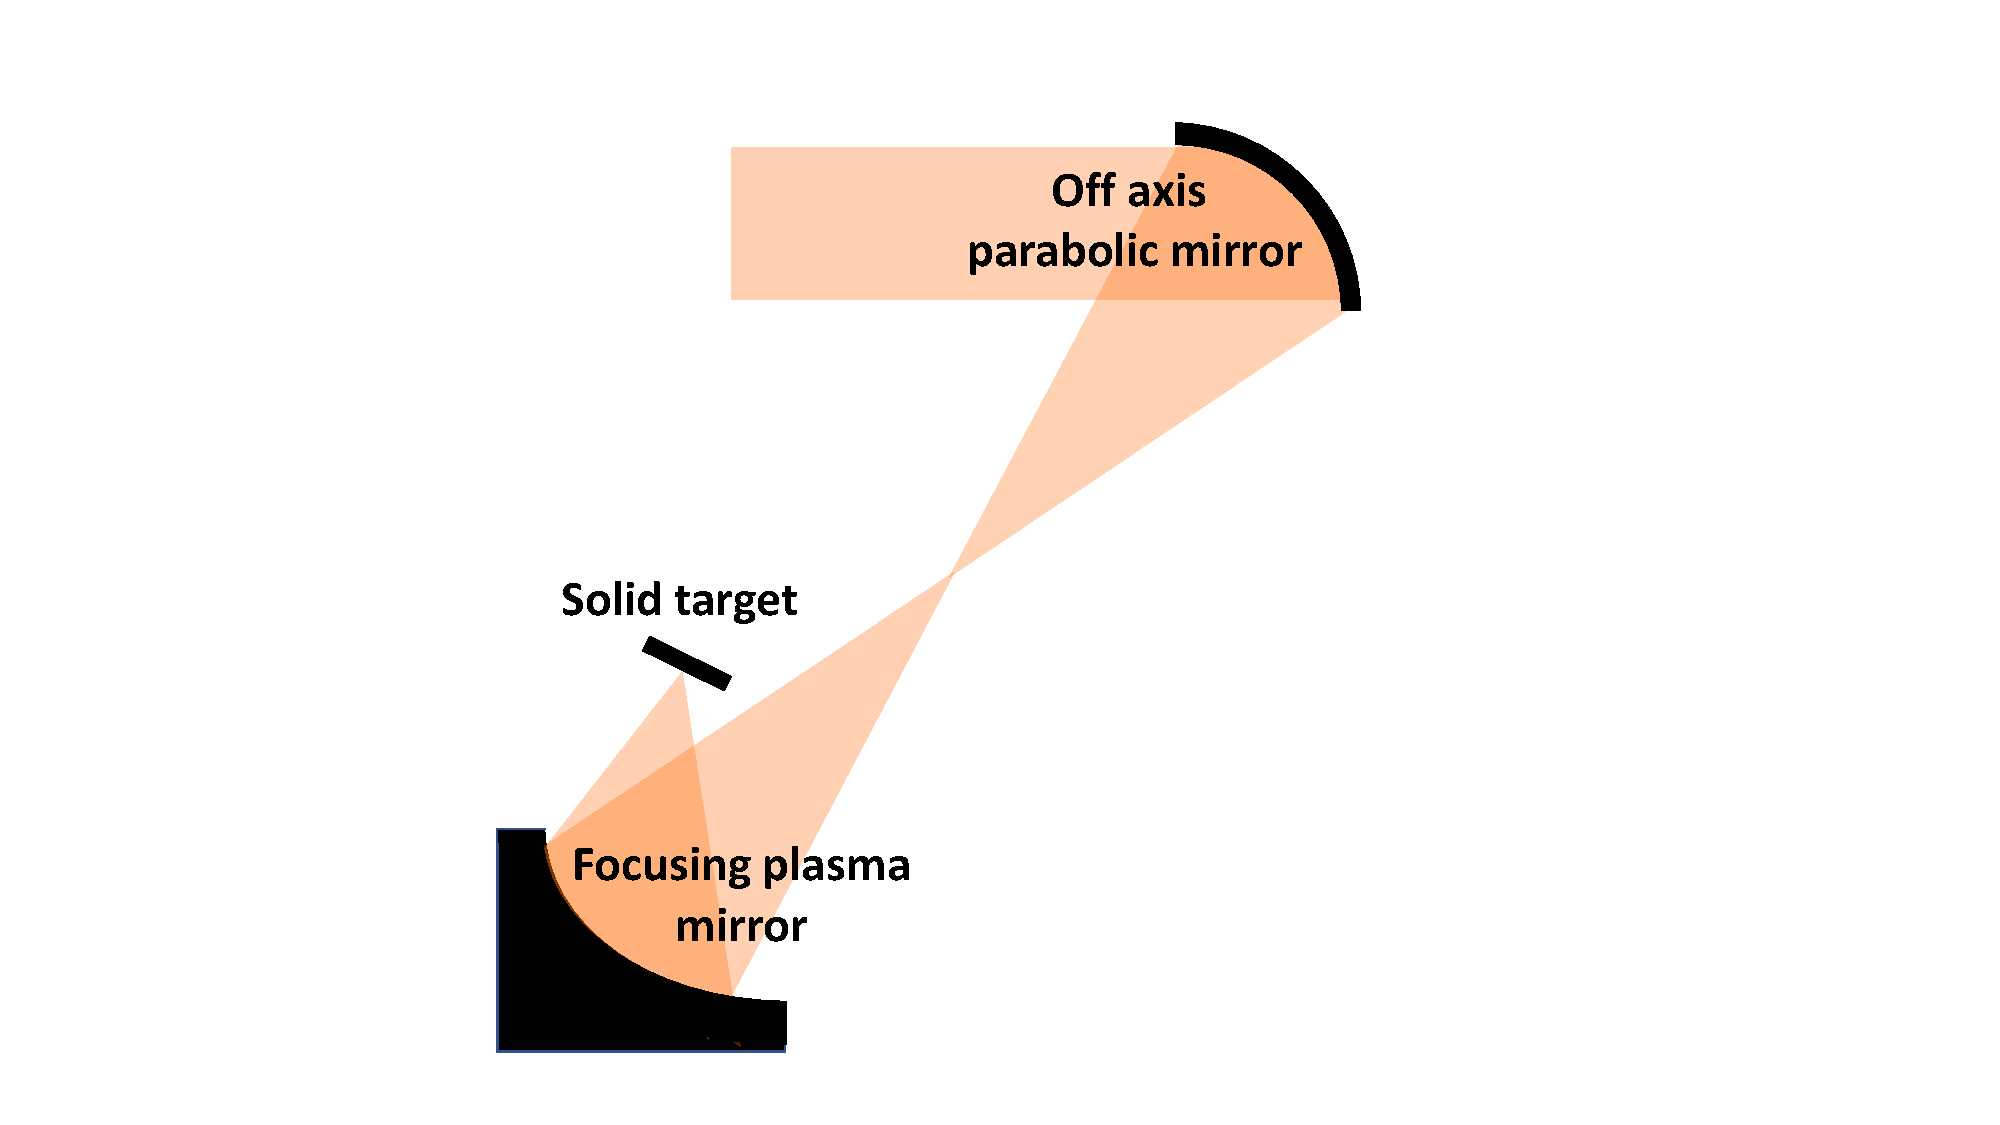
\includegraphics[width=0.35\linewidth]{./img/exp/diagram.pdf}}}
	\hspace{5mm}
	\sidesubfloat[]{{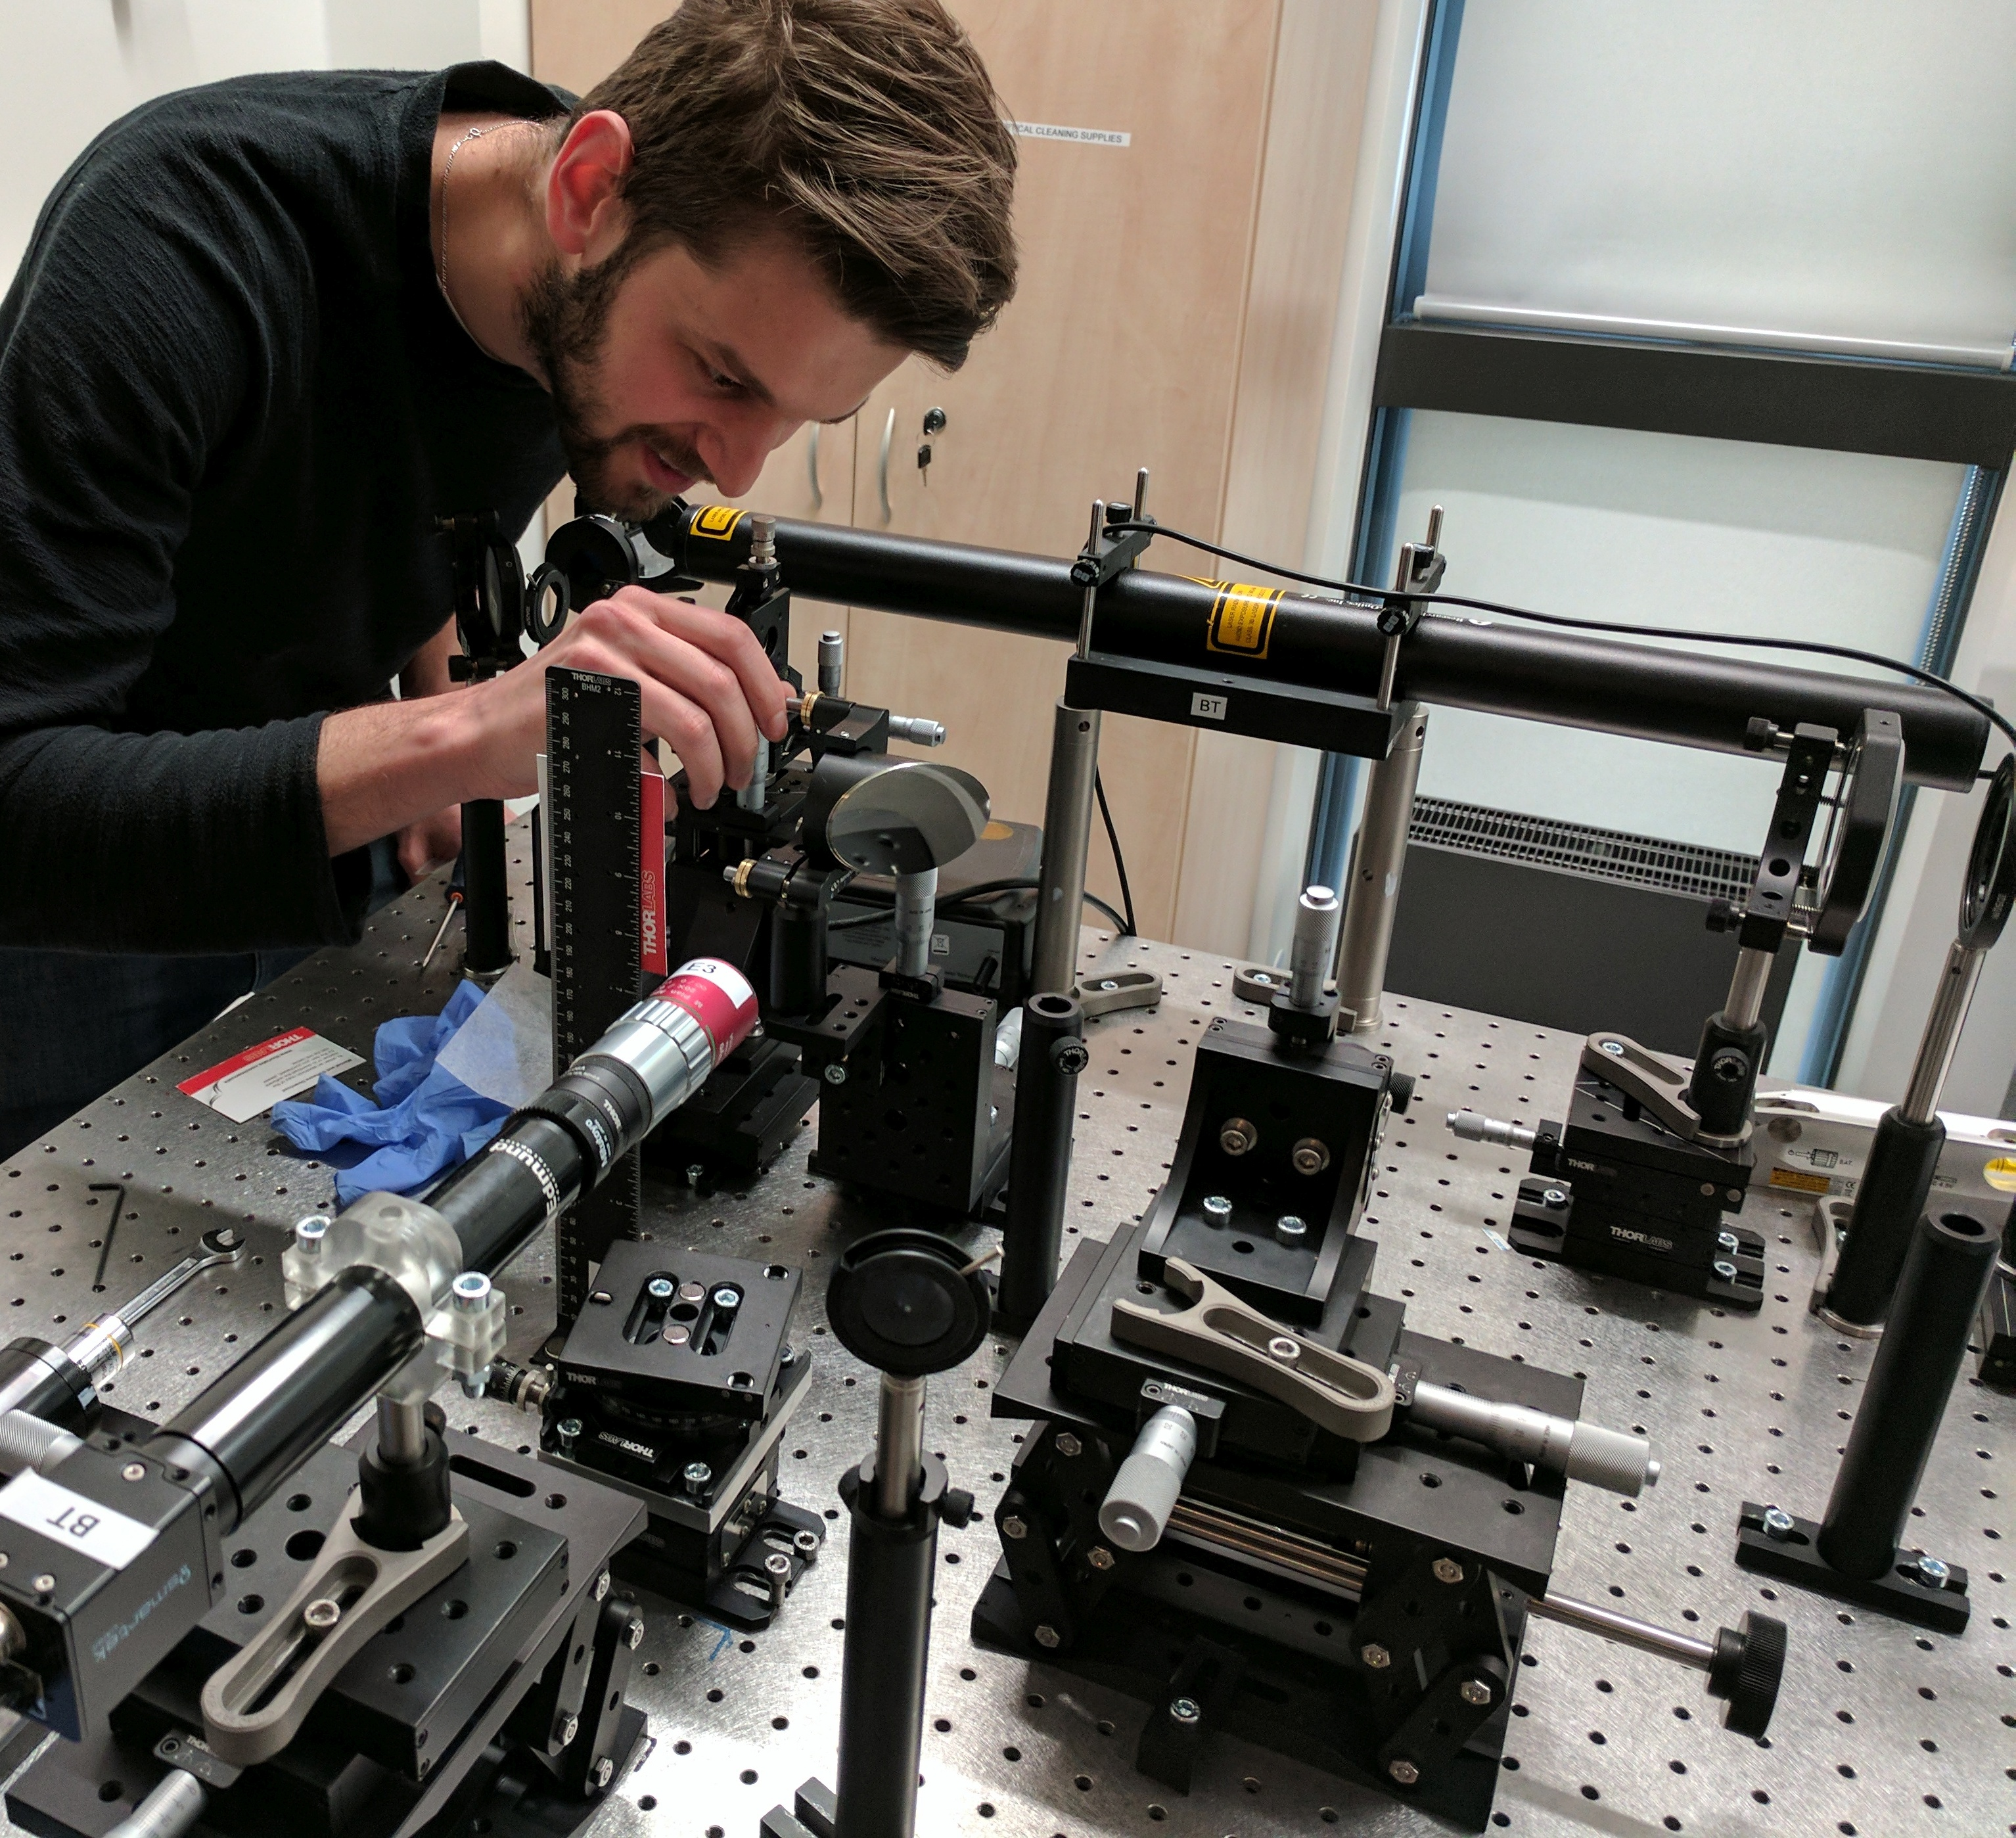
\includegraphics[width=0.4\linewidth]{./img/exp/photo2.jpg}}}
	\caption{}
	\label{}
\end{figure}